

\subfile{../journal/Tage/2024-07-03.tex}

\subsubchapter{Gaussian Probability Density Approximation}
Since for one loop diagrams we encounter at max a combination of two $\drho_{R_\omega}$ measures, we can simply take its average using the gained density $r_*\mapsto\exp(-\beta\cdot U(r_*))$. Looking at the two loop diagrams we have to do a bit of argumentation, since
\[
    (\text{Ex}_3(\mcL_f)\,Z_{z,R_\omega}^{(0)})[J] = \frac{1}{6}\cdot\bbra{
        \mcL_{f,mcF,\overline{\text{II}}} + \mcL_{f,\mcF.\overline{\text{III}}}
    }^3Z_{z,R_\omega}^{(0)}[J]
\] 
yields the measure
\[
    \bbra{(\square_{R_\omega})\otimes\drho_{R_\omega}}\otimes\bbra{(\square_{R_\omega})\otimes\drho_{R_\omega}}\otimes\bbra{(\square_{R_\omega})\otimes\drho_{R_\omega}}.
\]
As for the fourth order $\bbra{\text{Ex}_4(\mcL_f)\,Z_{z,R_\omega}^{(0)}[J]}$ there appear four total $\drho_{R_\omega}$ measures in the same product, and so on. Since there is an integration to be made over all $\omega\in\Omega$, i.e. $e^{-\beta\cdot H(r,\phi)}\cdot\uplambda(d(r,\phi))$ with regard to the particle positions $r$, we need to eventually calculate
\[
    \int_{V_{d,N}}\bbra{(\square_{R_\omega})\otimes\drho_{R_\omega}}^n\cdot\bbra{\exp(U)\cdot\uplambda}(d(r_*)),\quad n>2.
\]
Because the mapping $r_*\mapsto e^{-\beta\cdot U(r_*)}$ is generally not of gaussian form $x\mapsto \exp(-\scpr{A\cdot x}{x}/2)$, we need to perform an approximation that has not been necessary before for the apriori density $r_*\mapsto 1/\abs{V_{d,N}}$. For this we refer to the work of Gavin E. Crooks and David Chandler in \cite{PhysRevE.56.4217}, which states for the hard sphere model that for medium densitys $\rho_*$ the probability measure $\mbbP_N$ for $N\in\N$ particles has the approximative density function $x\mapsto \exp(-\scpr{A\cdot (x - \nu_{\text{MC}})}{x - \nu_{\text{MC}}}/(2\cdot\sigma_{\text{MC}}))$, where $\nu_{\text{MC}}$ and $\sigma_{\text{MC}}$ respectively are expected values and standard deviations of a Monte Carlo simulation. Hereby we suggest making an error by approximation of the correct density $r_*\mapsto\exp(-\beta\cdot U(r_*))$ with a gaussian density:
\[
    \exp(-\beta\cdot U(r_*))\approx\exp(-\scpr{A\cdot (r_* - \nu_{\text{MC}})}{r_* - \nu_{\text{MC}}}/(2\cdot\sigma_{\text{MC}})),
\]
This means that the theorem of Isserlis/Wick can be applied to the probability density of particle positions and our result $\overline{\hat\drho_{R_\omega}(q)\cdot\hat\drho_{R_\omega}(-q)} = S_*(q)/\rho_*$ can be applied. Figure \ref{fig:GaussianDensityFig} shows in subfigure \ref{fig:GaussianDensityFig1} the values of $\mbbP_N(V)$ for various diameters $2.0\sigma$ to $4.0\sigma$ at a fixed density of $0.5$. It can be seen that for all diameters the distribution nearly follows a gaussian form. The diameter $2.0$ furthermore corresbonds to the exclusion volume of the hard sphere model, i.e. the volume in which no other particle can be found. On the other hand, the largest volume $4.0\sigma$ is $64$ times as large as that of one particle. Subfigure \ref{fig:GaussianDensityFig2} varies the density from $0.1$ to $0.9$ at a fixed volume diameter of $3.5\sigma$. One can clearly see deviations for high and low densities from the gaussian form \cite{PhysRevE.56.4217}.
\begin{figure}[H]
    \centering
    \begin{subfigure}[b]{0.45\textwidth}
        \centering
        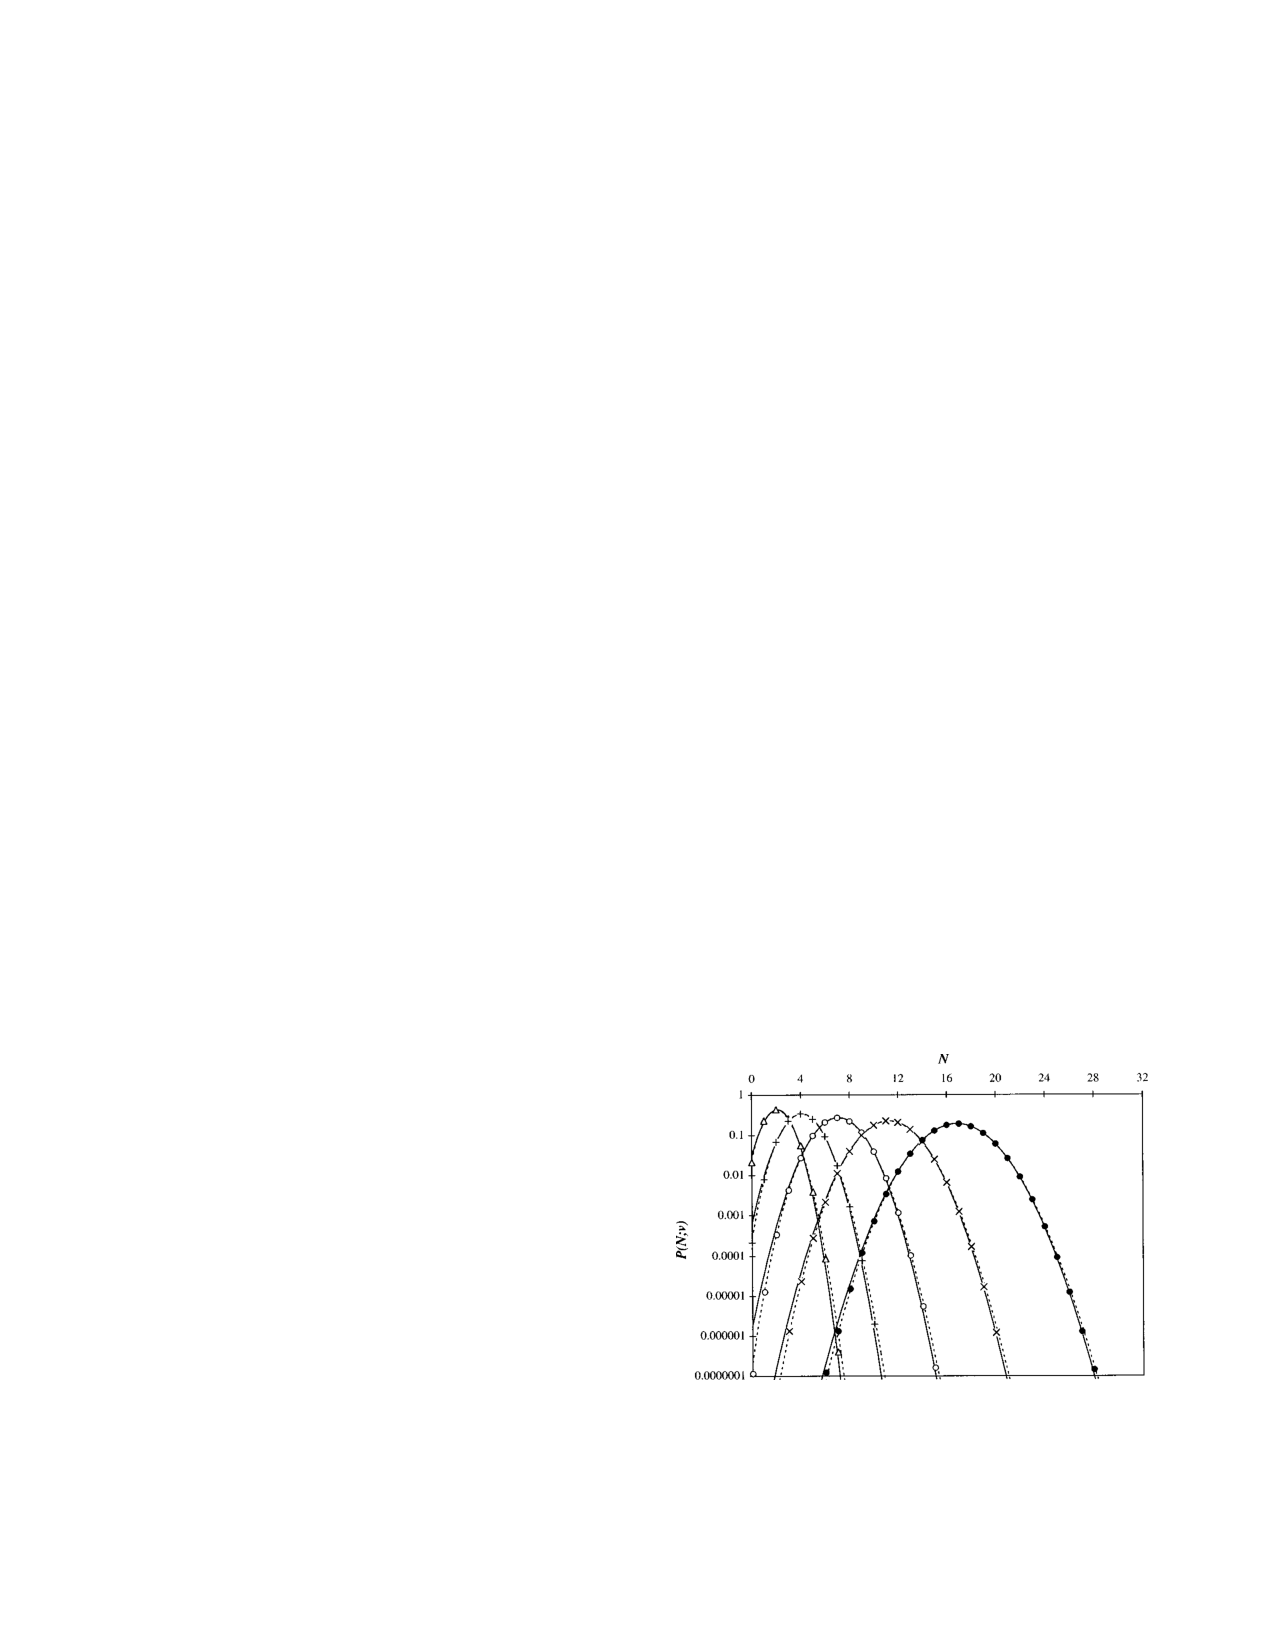
\includegraphics[width=\textwidth]{Inhalt/pdfs/GaussianDensityFig1.pdf}
        \caption{Diameters $2.0\sigma\;(\trangle)$, $2.5\sigma\;(+)$, $3.0\sigma\;(\bigcirc)$, $3.5\sigma\;(\times)$ and $4.0\sigma\;(\bullet)$. Density is $0.5$.}
        \label{fig:GaussianDensityFig1}
    \end{subfigure}
    \
    \begin{subfigure}[b]{0.45\textwidth}
        \centering
        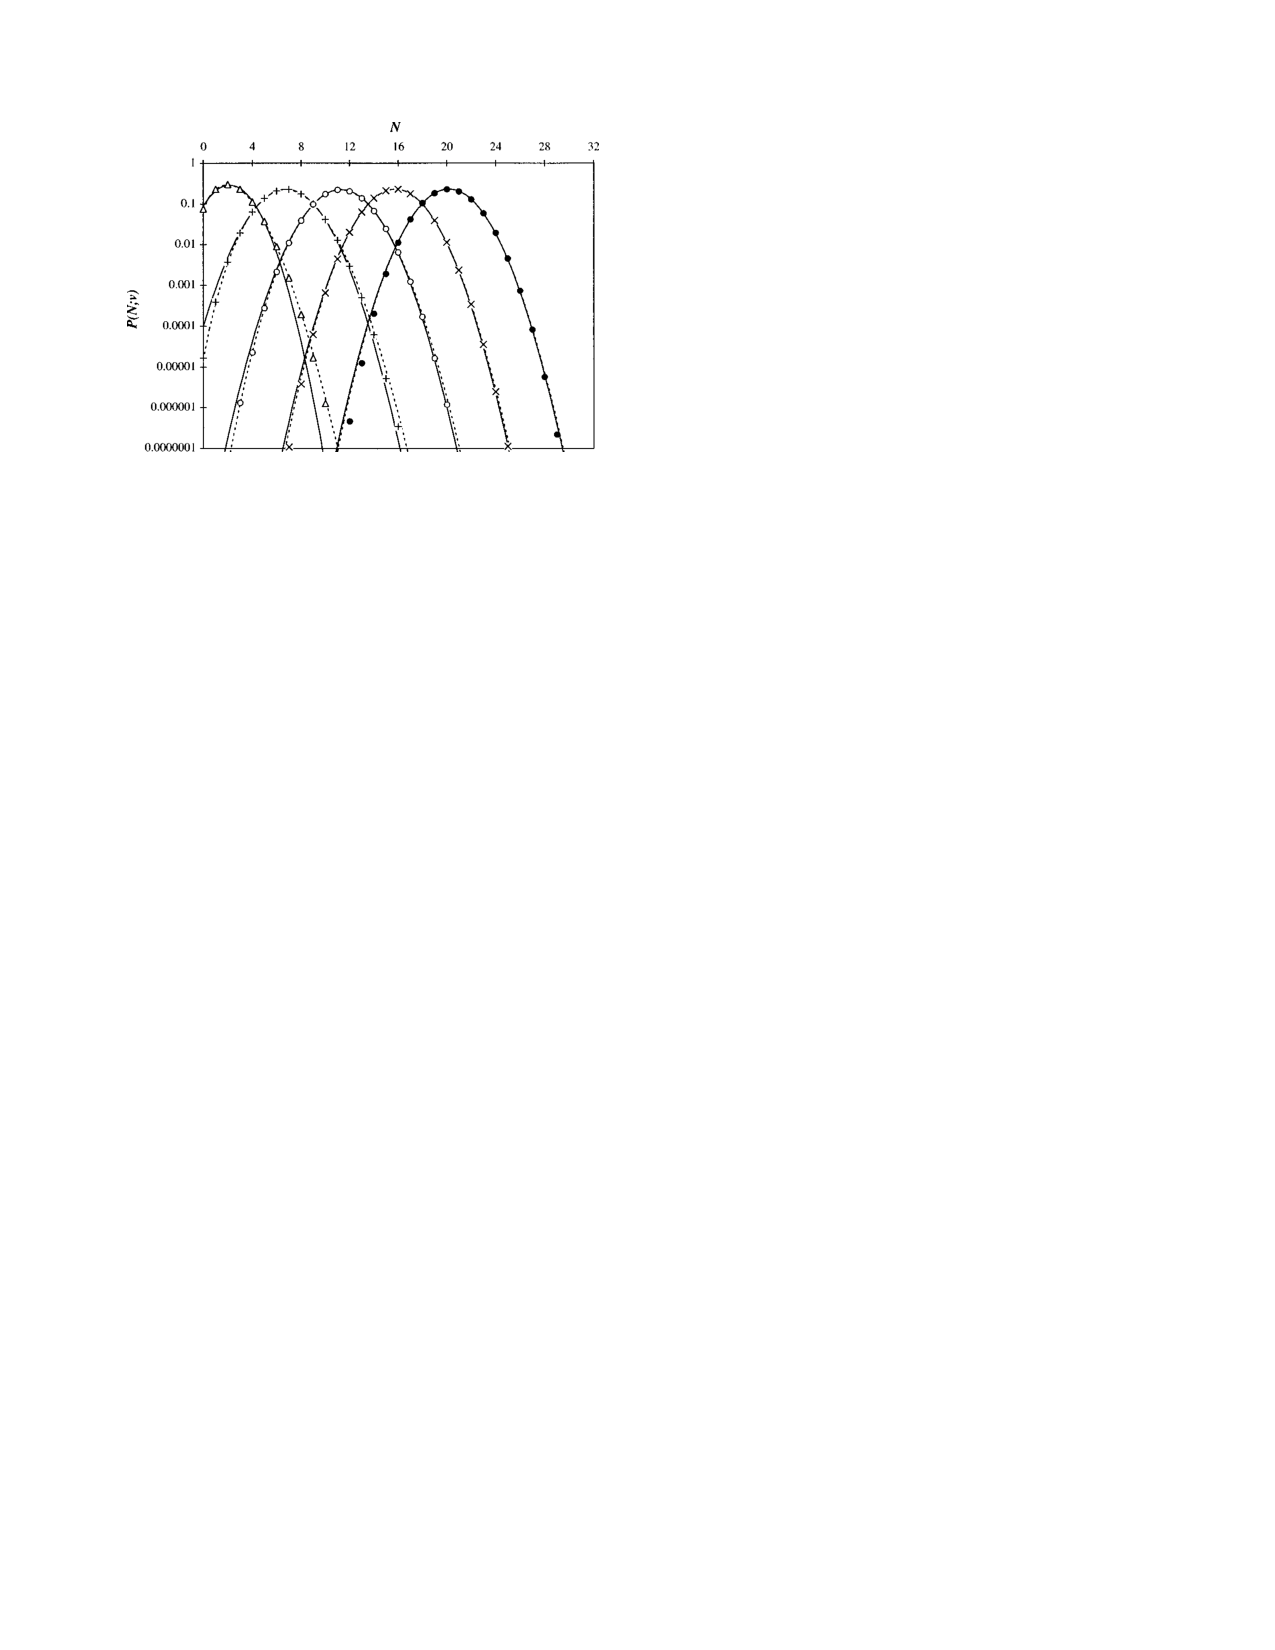
\includegraphics[width=\textwidth]{Inhalt/pdfs/GaussianDensityFig2.pdf}
        \caption{Diameter is $3.5\sigma$. Density varies from $0.1$ to $0.9$ following $0.1\;(\trangle)$, $0.3\;(+)$, $0.5\;(\bigcirc)$, $0.7\;(\times)$ and $0.9\;(\bullet)$.} 
        \label{fig:GaussianDensityFig2}
    \end{subfigure}
    \caption{Values of $\mbbP_N(V)$ for spherical volumes $V_\sigma$ for finding $N$ particles within. The points were gained by computer simulation, lines follow a gaussian distribution.}
    \label{fig:GaussianDensityFig}
\end{figure}

\subsubchapter{Relation to other Correlation Approaches}
As we have mentioned in the beginning, there was another approach made towards the implementation of correlated disorder into the ERM model by Martin-Mayor in \cite{10.1063/1.1349709}. In chapter IV of his work he introduces a method to implement a Gibbs distribution (in our wording also known as Boltzmann distribution) into the ERM model. It is achieved by multiplication with the corresponding measure, in our case the Lebesgue measure $\uplambda$. This yields a modified particle probability measure
\[
    \frac{1}{\abs{V_{d,N}}}\cdot\exp(-\beta\cdot U(r))\cdot\uplambda(dr).
\]
One immediately notices the similarity to our approach, where we have also used an exponetial density $r\mapsto \exp(-\beta\cdot U(r))$. Hereby we have introduced $U$ as being a sum of pair potential functions, from which we have been able to deduce
\[
    \exp(-\beta\cdot U(r)) = \exp(-\beta\cdot\frac{1}{2}\cdot\sum_{i,j\in[N]_{\neq}}u(r_i - r_j)) = \prod_{i,j\in[N]_{\neq}}\exp(-\beta\cdot u(r_i - r_j)/2).
\]
The difference to Martin-Mayor's now is twofold, as we did not consider an extra normalization factor of $1/\abs{V_{d,N}}$ in our density and our summation includes more particle connections than the \emph{superposition approximation} done in \cite{10.1063/1.1349709}. It only considers direct neighbors in a chained fashion, such that the summation would be 
\[
    \exp(-\beta\cdot U(r)) \stackrel{\cite{10.1063/1.1349709}}{=} \frac{1}{\abs{V_{d,N}}}\cdot\exp(-\beta\cdot\sum_{i\in[N-1]}u(r_i - r_{i+1})) = \frac{1}{\abs{V_{d,N}}}\cdot\prod_{i\in[N-1]}\exp(-\beta\cdot u(r_i - r_{i+1})).
\]
Despite the neglect of furher correlations, Martin-Mayor's approach was tested in the context of supercooled liquids in the calculation of coupling coefficients and mode coupling theory. The results were found to be reasonably accurate \cite{10.1063/1.1349709}. \\

Furthermore the paper suggests that the density in superposition approximation can be included into the spring function iteslf, by defining $\mcf(r) := \exp(-\beta\cdot u(r))\cdot f(r)/\abs{V_{d,N}}$ for $f(r)$ being the spring function. It is claimed that in the lowest order this would lead to the bare propagator having the form
\[
    G_0^{(\mathit{MM})}(\vp,z) = \Bbra{
        z - \rho_*\cdot\bbra{\hat\mcf(0) - \hat\mcf(\vp)}
    }^{-1}.
\]
In our approach this is not the case, as the zeroth order perturbation theory is not affected by the introduced structure factor and therefore remains unchanged. 
